\documentclass{article}
\usepackage[T1]{fontenc}
\usepackage[scaled]{helvet}
\usepackage{tikz}
\usepackage[margin=0.45in,landscape]{geometry}
\usepackage{graphicx}
\usetikzlibrary{arrows.meta,positioning,fit,backgrounds}
\pagestyle{empty}
\renewcommand{\familydefault}{\sfdefault}

\begin{document}
\centering
\resizebox{\textwidth}{0.80\textheight}{%
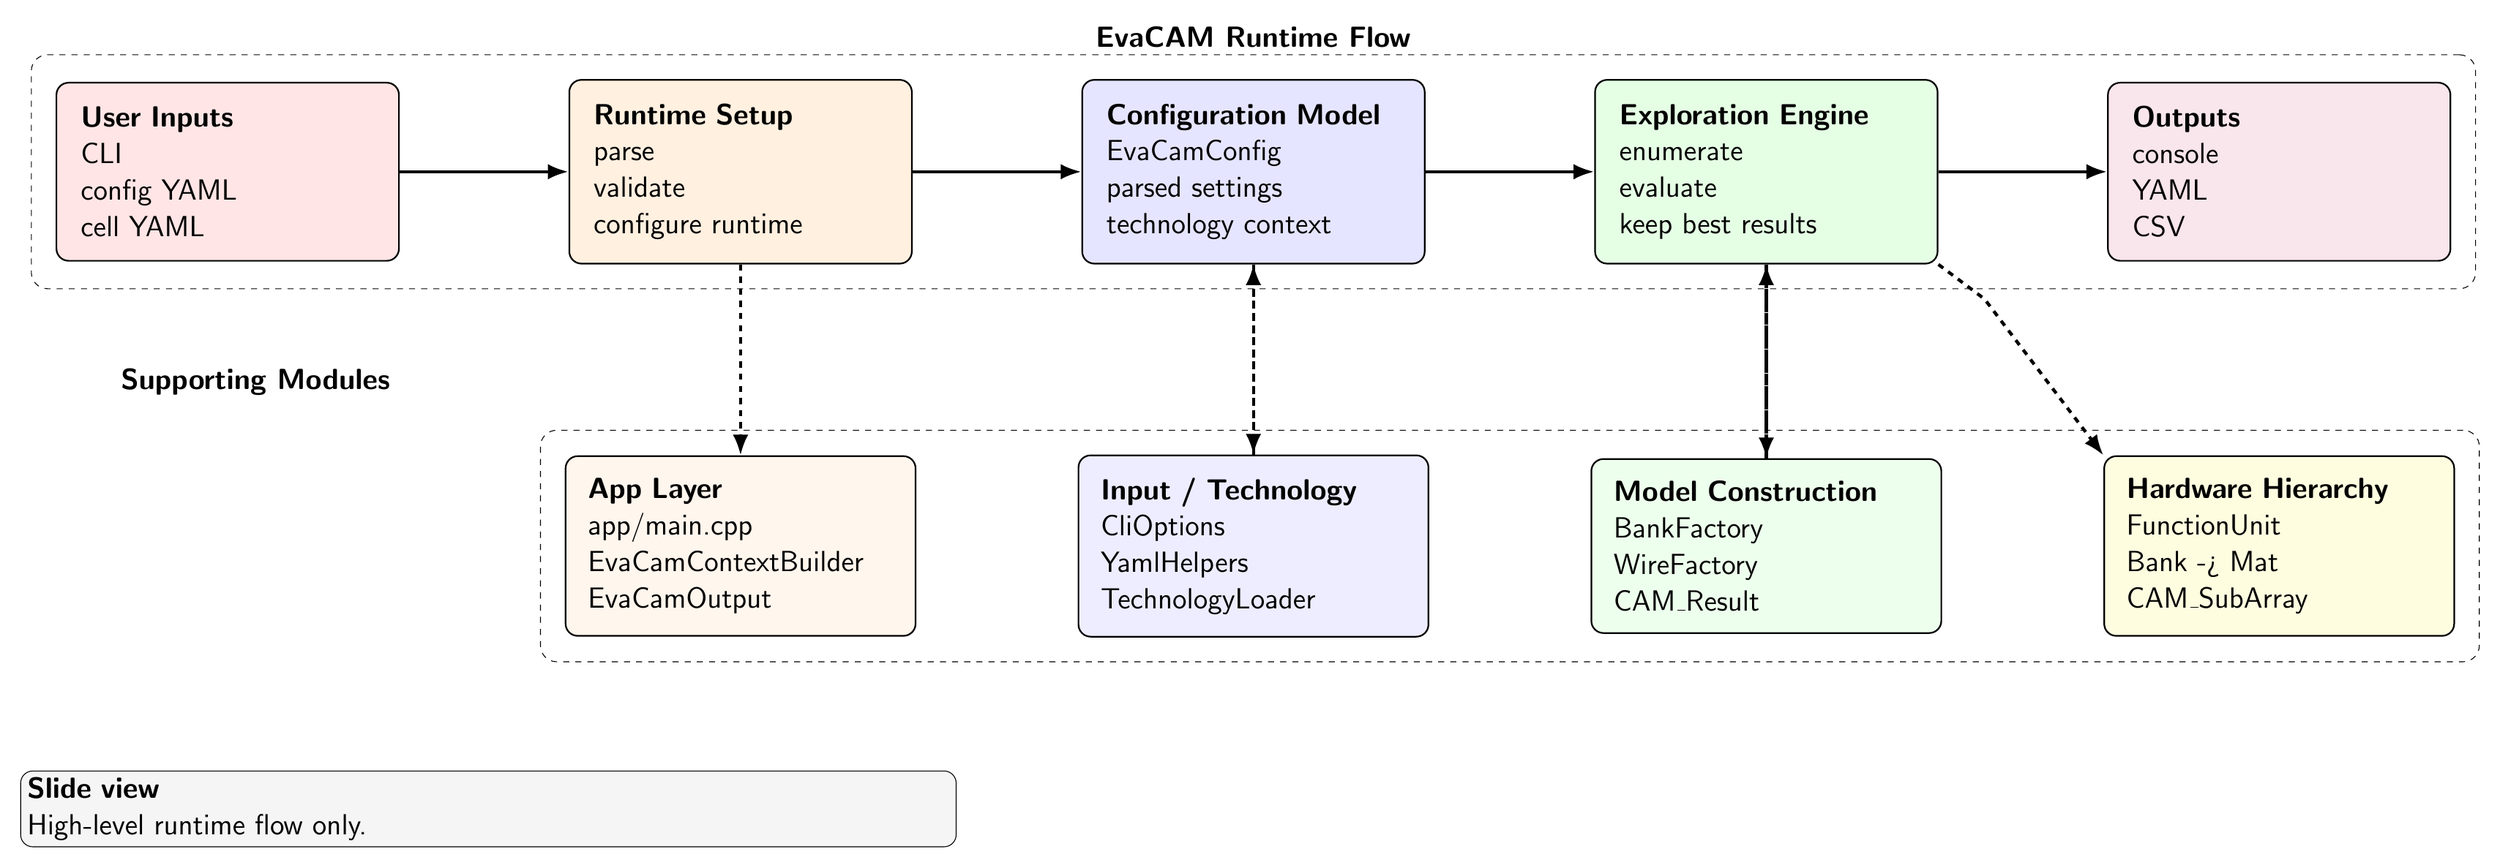
\begin{tikzpicture}[
  font=\Large,
  >=Latex,
  stage/.style={
    draw,
    rounded corners=6pt,
    align=left,
    minimum width=5.7cm,
    minimum height=2.8cm,
    text width=5.1cm,
    inner sep=12pt,
    thick,
    fill=white
  },
  support/.style={
    draw,
    rounded corners=6pt,
    align=left,
    minimum width=5.9cm,
    minimum height=2.2cm,
    text width=5.3cm,
    inner sep=11pt,
    thick,
    fill=white
  },
  group/.style={
    draw,
    dashed,
    rounded corners=8pt,
    inner sep=12pt
  },
  flow/.style={-Latex, ultra thick},
  link/.style={-Latex, ultra thick, dashed}
]

% Main flow
\node[stage, fill=red!10] (input) at (-14.0, 0.3) {%
  \textbf{User Inputs}\\
  CLI\\
  config YAML\\
  cell YAML
};

\node[stage, fill=orange!12] (context) at (-5.1, 0.3) {%
  \textbf{Runtime Setup}\\
  parse\\
  validate\\
  configure runtime
};

\node[stage, fill=blue!10] (config) at (3.8, 0.3) {%
  \textbf{Configuration Model}\\
  EvaCamConfig\\
  parsed settings\\
  technology context
};

\node[stage, fill=green!10] (explore) at (12.7, 0.3) {%
  \textbf{Exploration Engine}\\
  enumerate\\
  evaluate\\
  keep best results
};

\node[stage, fill=purple!10] (output) at (21.6, 0.3) {%
  \textbf{Outputs}\\
  console\\
  YAML\\
  CSV
};

% Support band
\node[support, fill=orange!7] (app) at (-5.1, -6.2) {%
  \textbf{App Layer}\\
  app/main.cpp\\
  EvaCamContextBuilder\\
  EvaCamOutput
};

\node[support, fill=blue!7] (loaders) at (3.8, -6.2) {%
  \textbf{Input / Technology}\\
  CliOptions\\
  YamlHelpers\\
  TechnologyLoader
};

\node[support, fill=green!7] (model) at (12.7, -6.2) {%
  \textbf{Model Construction}\\
  BankFactory\\
  WireFactory\\
  CAM\_Result
};

\node[support, fill=yellow!12] (hardware) at (21.6, -6.2) {%
  \textbf{Hardware Hierarchy}\\
  FunctionUnit\\
  Bank -> Mat\\
  CAM\_SubArray
};

% Flow arrows
\draw[flow] (input) -- (context);
\draw[flow] (context) -- (config);
\draw[flow] (config) -- (explore);
\draw[flow] (explore) -- (output);

% Support links
\draw[link] (context) -- (app);
\draw[link] (config) -- (loaders);
\draw[link] (explore) -- (model);
\draw[link] (explore.south east) -- ++(0.8,-0.6) -- (hardware.north west);

% Extra narrative links
\draw[link] (loaders.north) -- (config.south);
\draw[link] (model.north) -- (explore.south);

% Group boxes
\node[group, fit=(input)(context)(config)(explore)(output), label=above:{\textbf{EvaCAM Runtime Flow}}] {};
\node[group, fit=(app)(loaders)(model)(hardware)] (supportGroup) {};
\node[fill=white, inner sep=4pt, anchor=west] at (-16.0, -3.35) {\textbf{Supporting Modules}};

% Footer note
\node[draw, rounded corners=6pt, fill=gray!8, align=left, anchor=north west, text width=16.0cm] at (-17.6, -10.1) {%
  \textbf{Slide view}\\
  High-level runtime flow only.
};

\end{tikzpicture}
}
\end{document}
